\begin{frame}{}
    \LARGE GANs: \textbf{Objective function}
\end{frame}

\begin{frame}[allowframebreaks]{Understanding the Objective function}
The goal of GANs is to find a \textbf{Nash equilibrium} between the generator and discriminator. 
The generator tries to minimize the probability of the discriminator correctly classifying fake data.
\begin{figure}
    \centering
    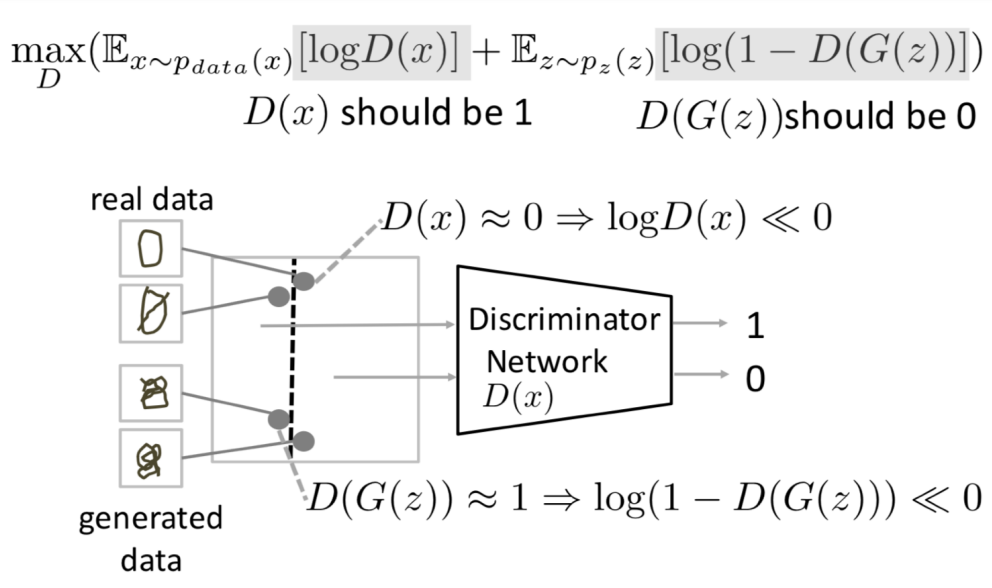
\includegraphics[height=0.7\textheight, width=\textwidth, keepaspectratio]{images/gan/gan_cost_1.png}
\end{figure}

\framebreak
\begin{figure}
    \centering
    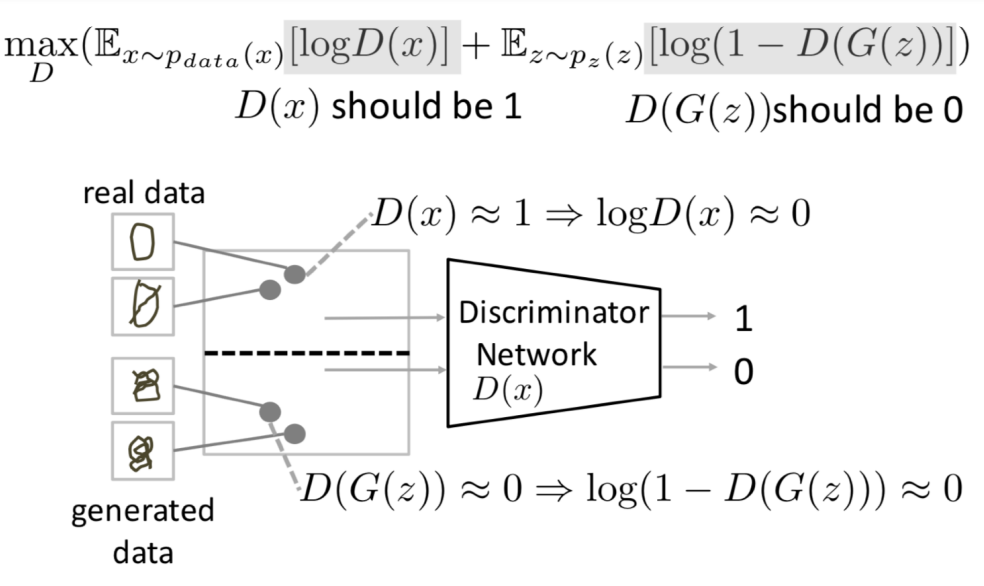
\includegraphics[height=0.9\textheight, width=\textwidth, keepaspectratio]{images/gan/gan_cost_2.png}
\end{figure}

\framebreak
\begin{figure}
    \centering
    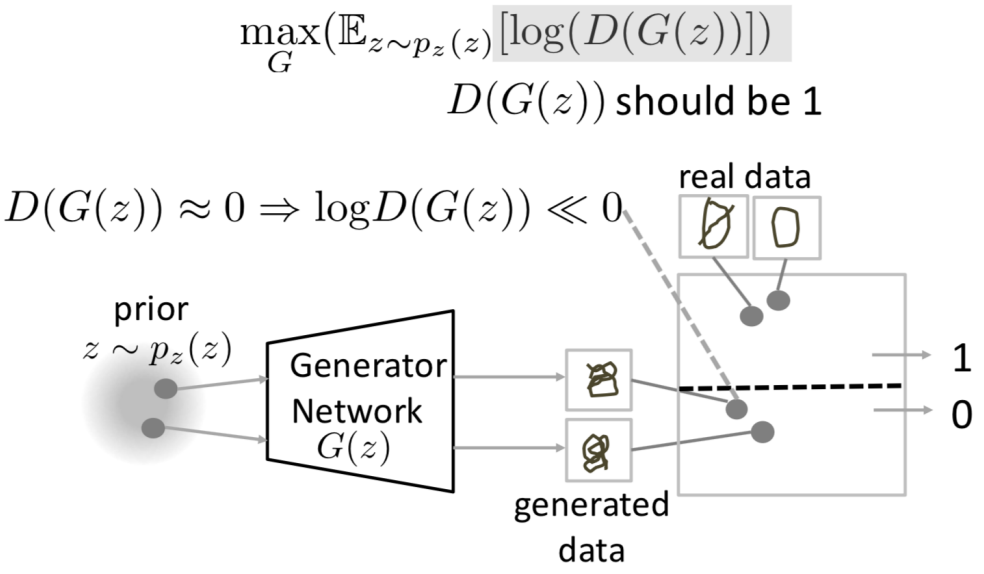
\includegraphics[height=0.9\textheight, width=\textwidth, keepaspectratio]{images/gan/gan_cost_3.png}
\end{figure}

\framebreak
\begin{figure}
    \centering
    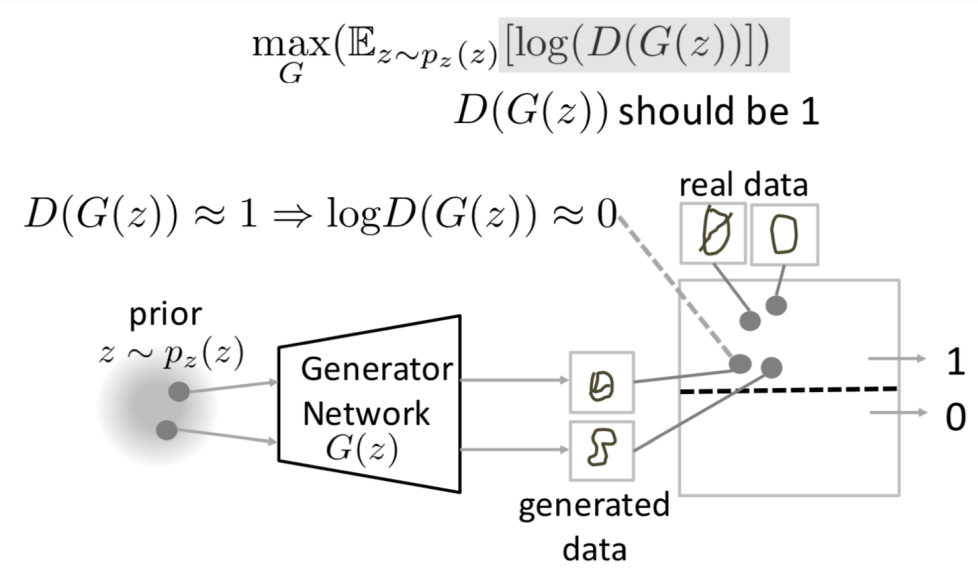
\includegraphics[height=0.9\textheight, width=\textwidth, keepaspectratio]{images/gan/gan_cost_4.png}
\end{figure}

\framebreak
\begin{figure}
    \centering
    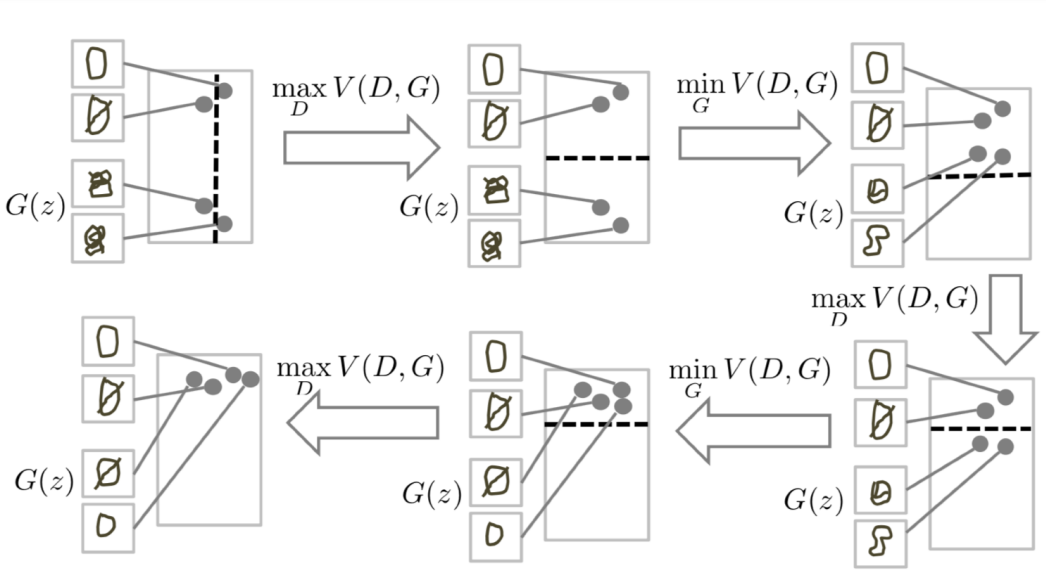
\includegraphics[height=0.9\textheight, width=\textwidth, keepaspectratio]{images/gan/gan_cost_5.png}
\end{figure}


\footnotetext{https://www.slideshare.net/ckmarkohchang/generative-adversarial-networks}
\end{frame}

\begin{frame}{GANs - Interactive Demo}
\centering
\href{https://poloclub.github.io/ganlab/}{https://poloclub.github.io/ganlab/}
    
\end{frame}